% This file was created by matlab2tikz.
%
\documentclass[tikz]{standalone}
\usepackage[T1]{fontenc}
\usepackage[utf8]{inputenc}
\usepackage{pgfplots}
\usepackage{grffile}
\pgfplotsset{compat=newest}
\usetikzlibrary{plotmarks}
\usepgfplotslibrary{patchplots}
\usepackage{amsmath}

\newlength\figureHeight \setlength{\figureHeight}{6cm}
\newlength\figureWidth \setlength{\figureWidth}{10cm}
\begin{document}
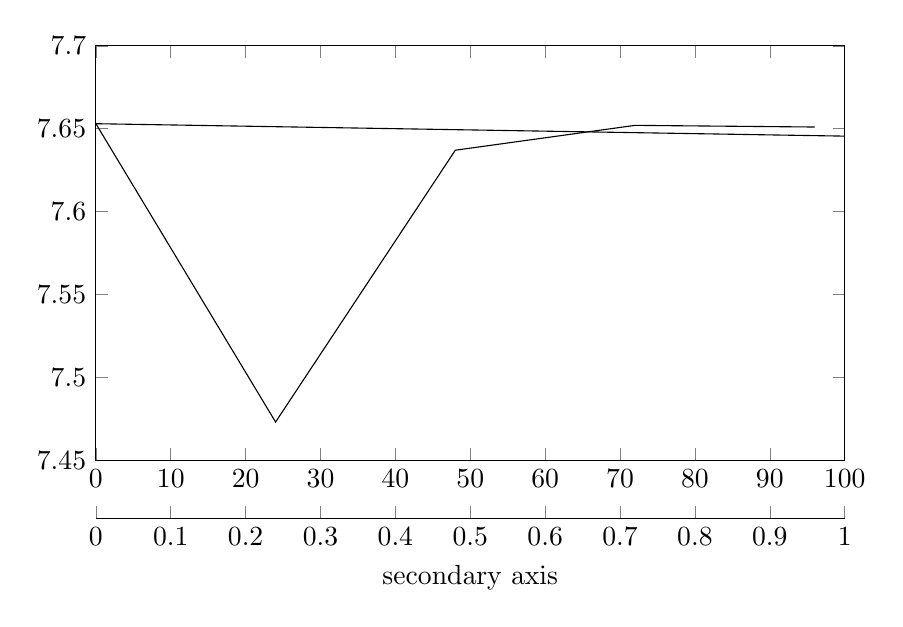
\begin{tikzpicture}

\begin{axis}[%
width=0.951\figureWidth,
height=0.877\figureHeight,
at={(0\figureWidth,0.123\figureHeight)},
scale only axis,
xmin=   0,
xmax= 100,
ymin=7.45,
ymax= 7.7,
axis background/.style={fill=white}
]
\addplot [color=black,solid,forget plot]
  table[row sep=crcr]{%
   0	7.653\\
  24	7.473\\
  48	7.637\\
  72	7.652\\
  96	7.651\\
};
\end{axis}

\begin{axis}[%
width=0.951\figureWidth,
height=0.877\figureHeight,
at={(0\figureWidth,0.123\figureHeight)},
scale only axis,
xmin=   0,
xmax=   1,
ymin=7.45,
ymax= 7.7,
hide axis
]
\addplot [color=black,solid,forget plot]
  table[row sep=crcr]{%
   0	7.653\\
 1.1	7.64475\\
};
\end{axis}

\begin{axis}[%
width=0.951\figureWidth,
height=0.012\figureHeight,
at={(0\figureWidth,0\figureHeight)},
scale only axis,
every outer x axis line/.append style={black},
every x tick label/.append style={font=\color{black}},
xmin=   0,
xmax=   1,
xminorticks=true,
xlabel={secondary axis},
every outer y axis line/.append style={white},
every y tick label/.append style={font=\color{white}},
ymin=   0,
ymax=   1,
ytick={\empty},
axis x line*=bottom,
axis y line*=left
]
\end{axis}
\end{tikzpicture}%
\end{document}